\documentclass[12pt]{article}
 
\newenvironment{sol}[1][Solution]{\begin{trivlist}\item[\hskip\labelsep {\bfseries #1:}]}{\end{trivlist}}
\usepackage{minted}
%\usemintedstyle{perldoc}
\usemintedstyle{vs}
\usepackage{graphicx}
\graphicspath{./}

\usepackage[margin=1in]{geometry} 
\usepackage{amsmath,amsthm,amssymb}
\usepackage{times,url}
\usepackage{tikz}
\usepackage{color}
\usepackage{enumerate}
\begin{document}
\renewcommand{\qedsymbol}{\filledbox}
\begin{center}
    \textbf{CS 5/7350 - Test\#3} \\
    \textbf{Fall, 2021}
%replace X with the appropriate number
\end{center}
\begin{flushright}
Name: \underline{Bingying Liang }\\
ID:  \underline{\ \ \ \ \ 48999397 \ \ \ \ \ }
\end{flushright}
\begin{enumerate}
    \item \ [6 pts] If a smallest last ordering has the largest degree when deleted of 15 and a terminal clique size of 12.
    \begin{enumerate}
        \item What is the maximum number of colors that might be required by the ordering?
        \begin{sol}
            16
        \end{sol}
        \item What is the minimum number of colors that must be required by the graph?
        \begin{sol}
            12
        \end{sol}
    \end{enumerate}

    \item \ [6 pts] When performing a BB84 key exchange, the person sending generates random 1’s and 0’s to send. Give two reasons this person should not just send the confidential file instead of random 1’s and 0’s?
    \begin{enumerate}
        \item Reason 1:
        \begin{sol}
            
        \end{sol}
        \item Reason 2:
        \begin{sol}
            Not on Test 3
        \end{sol}
    \end{enumerate}

    \item \ [10 pts] Consider the following NP completeness questions. Answer them with the best answer of “some” “all” “none” or “unknown”
    \begin{enumerate}
        \item Which Problems in NP are also in P? (“some” “all” “none” or “unknown”)
        \begin{sol}
            unknown
        \end{sol}
        \item Which Problems in P are also in NP? (“some” “all” “none” or “unknown”)
        \begin{sol}
            all
        \end{sol}
        \item Which Problems in NP-Hard are also in NP? ( “some” “all” “none” )
        \begin{sol}
            some
        \end{sol}
        \item Which Problems in NP-Complete are in NP-Hard ( “some” “all” “none” or “unknown”)
        \begin{sol}
            all
        \end{sol}
        \item If someone can solve an NP-Complete problem in Polynomial Time, then all NP and all NP-Hard problems can be solved in polynomial time. (true or false)
        \begin{sol}
            false
        \end{sol}
        \item If someone can solve an NP-Complete problem in Polynomial Time, then all NP and all NP-Complete problems can be solved in polynomial time. (true or false)
        \begin{sol}
            true
        \end{sol}
        \item At least 1 NP problem can be solved in polynomial time? (True or False)
        \begin{sol}
            true
        \end{sol}
        \item NP-Complete problems are in P (“true” “false” or “unknown”)
        \begin{sol}
            unknown
        \end{sol}
        \item Which NP-Hard Problems are also NP-Complete? ( “some” “all” “none” or “unknown”)
        \begin{sol}
            some
        \end{sol}
        \item \textcolor{red}{To show a problem is NP-Complete, you must show it is NP and that a solver for another NP-Complete problem can solve it as well. (True or False)}
        \begin{sol}
            False\\
            Explain: To show a problem, Q, is NP-Complete, you must show Problem Q is NP and that a solver for problem Q can solve another NP-Hard problem.
        \end{sol}
    \end{enumerate}

    \item \ [6 pts] Using $n_0$ equal to 10, show that $f(n) = 8n^2 + 5n + 1$ is $O(n^3)$.
        \begin{sol}
                \begin{align*}
            O(n^3): & 0 \leq  f(n)\leq c_2g(n), \forall n = n_0 = 10\\
            & 8n^2 + 5n + 1\leq c_2 n^3, \forall n = n_0 = 10\\
            & \frac{8}{n} + \frac{5}{n^2} + \frac{1}{n^3} \leq  c_2 , \forall n = n_0 = 10\\
            & \frac{8}{10} + \frac{5}{10^2} + \frac{1}{10^3} \leq  c_2\\
            & 0.851 \leq c_2 \\
            & \therefore c_2 = 0.851 \text{ can let }f(n) \text{ is } O(n^3), \forall n = n_0 = 10 \\
        \end{align*}
    \end{sol}


    \item \ \textcolor{red}{[10 pts] Consider two different algorithms that each solve a different problem.}
    \begin{itemize}
        \item Implementation X solves Problem Px and Implementation X is $\Theta(n)$
        \item Implementation Y solves Problem Py and Implementation Y is $\Theta(2^n)$
    \end{itemize}
    Determine if each of these “Yes it is true”, “Maybe it is true but doesn’t have to be”, or “No it is not true”
    \begin{enumerate}
        \item Problem Px is harder than Problem Py
        \begin{sol}
            Maybe it is true but doesn’t have to be
        \end{sol}
        \item Problem Py is harder than Problem Px
        \begin{sol}
            Maybe it is true but doesn’t have to be
        \end{sol}
        \item Implementation X is harder than Implementation Y
        \begin{sol}
            No it is not true 
        \end{sol}
        \item Problem X is $\Omega(n)$
        \begin{sol}
            Maybe it is true but doesn’t have to be
        \end{sol}
        \item Problem X is $\omega(n)$
        \begin{sol}
             No it is not true
        \end{sol}
        \item Problem X is $O (n)$
        \begin{sol}
            Yes it is true
        \end{sol}
        \item Problem X is $o (n)$
        \begin{sol}
            Maybe it is true but doesn’t have to be
        \end{sol}
        \item Implementation X is $\Omega(n)$
        \begin{sol}
            Yes it is true
        \end{sol}
        \item Implementation X is $\omega (n)$.
        \begin{sol}
            No it is not true
        \end{sol}
        \item Implementation Y is $O(n^n)$
        \begin{sol}
            Yes it is true
        \end{sol}
    \end{enumerate}
    \item \textcolor{red}{ [4 pts] How many swaps in the worst case may be required to form a heap using the HEAPIFY algorithm from an array of 16 items?}
    \begin{sol}
        15
    \end{sol}

    \item \ [6 pts] Show the addition table required for addition that adds two numbers from the number system $\beta$ = 7 and D = \{ -3, -2, -1, 0, 1, 2, 3, 4, 5 \} giving a number in the same number system. Ensure the addition can be performed in parallel without having to “ripple” a carry. (You do not need to fill in the grey areas

    \begin{sol}
        Not on Test 3
    \end{sol}

    \item \ [8 pts] You have 3 dice. Each one is different.
    \begin{itemize}
        \item Die \#1 has sides \{ 0, 1, 2 \} with a
        \begin{itemize}
            \item 25\% chance of rolling a 0, a
            \item 35\% chance of rolling a 1 and a
            \item 40\% chance of rolling a 2.
        \end{itemize}
        \item Die \#2 has sides \{ 2, 2, 0 \} with a
        \begin{itemize}
            \item 30\% chance of rolling the first 2 and a
            \item 30\% chance of rolling the other 2 and a
            \item 40\% chance of rolling a 0
        \end{itemize}

        \item Die \#3 has sides \{0, 1\} with a
        \begin{itemize}
            \item 40\% chance of rolling a 0 and a
            \item 60\% chance of rolling a 1
        \end{itemize}
    \end{itemize}
    \begin{enumerate}
        \item Fill in the table for the dynamic programming algorithm to solve the problem.
        \begin{sol}
        \hspace*{\fill}
                                    \begin{center}
    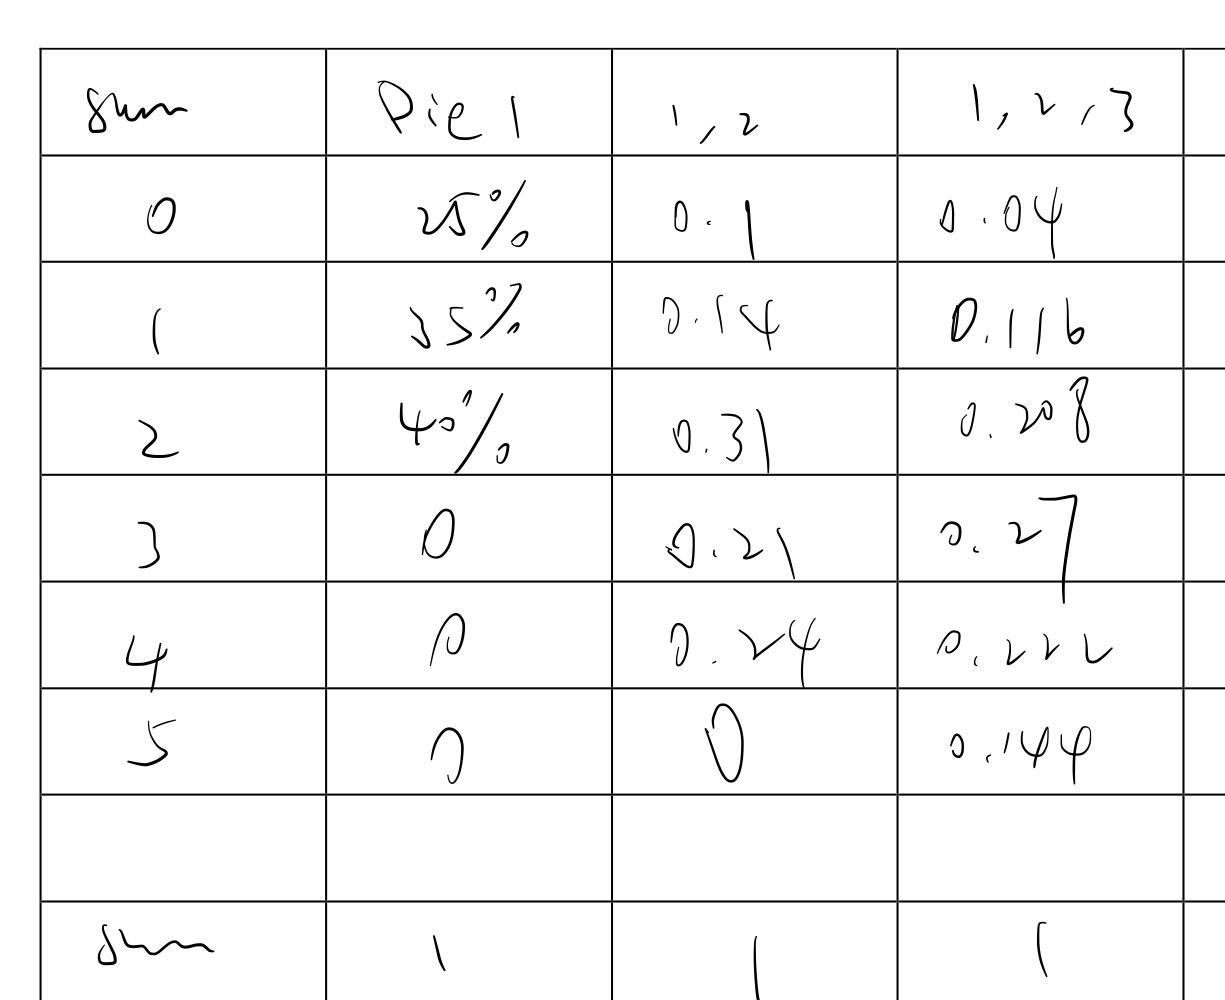
\includegraphics[width=0.6\textwidth]{p1.jpeg}
    \end{center} 
        \end{sol}
        \item What is the probability of rolling a 0?
        \begin{sol}
            0.04
        \end{sol}
        \item What is the probability of rolling a 1?
                \begin{sol}
            0.116
        \end{sol}
        \item What is the probability of rolling a 2?
                \begin{sol}
            0.208
        \end{sol}
        \item What is the probability of rolling a 3?
                \begin{sol}
            0.27
        \end{sol}
        \item What is the probability of rolling a 4?
                \begin{sol}
            0.222
        \end{sol}
        \item What is the probability of rolling a 5?
                \begin{sol}
            0.144
        \end{sol}
    \end{enumerate}

    \item \ [8 pts] Create a graph with a starting vertex of “S” (when required) where:
    \begin{enumerate}
        \item The weight of the third edge chosen with Prims Minimum Spanning Tree Algorithm is less than the weight of the third edge chosen with Kruskal’s Minimum Spanning Tree Algorithm. Mark the third edge chosen by prim’s algorithm with a “P” and the third edge chosen by Kruskal’s algorithm with a “K”.
        \begin{sol}
        \hspace*{\fill}
                                    \begin{center}
    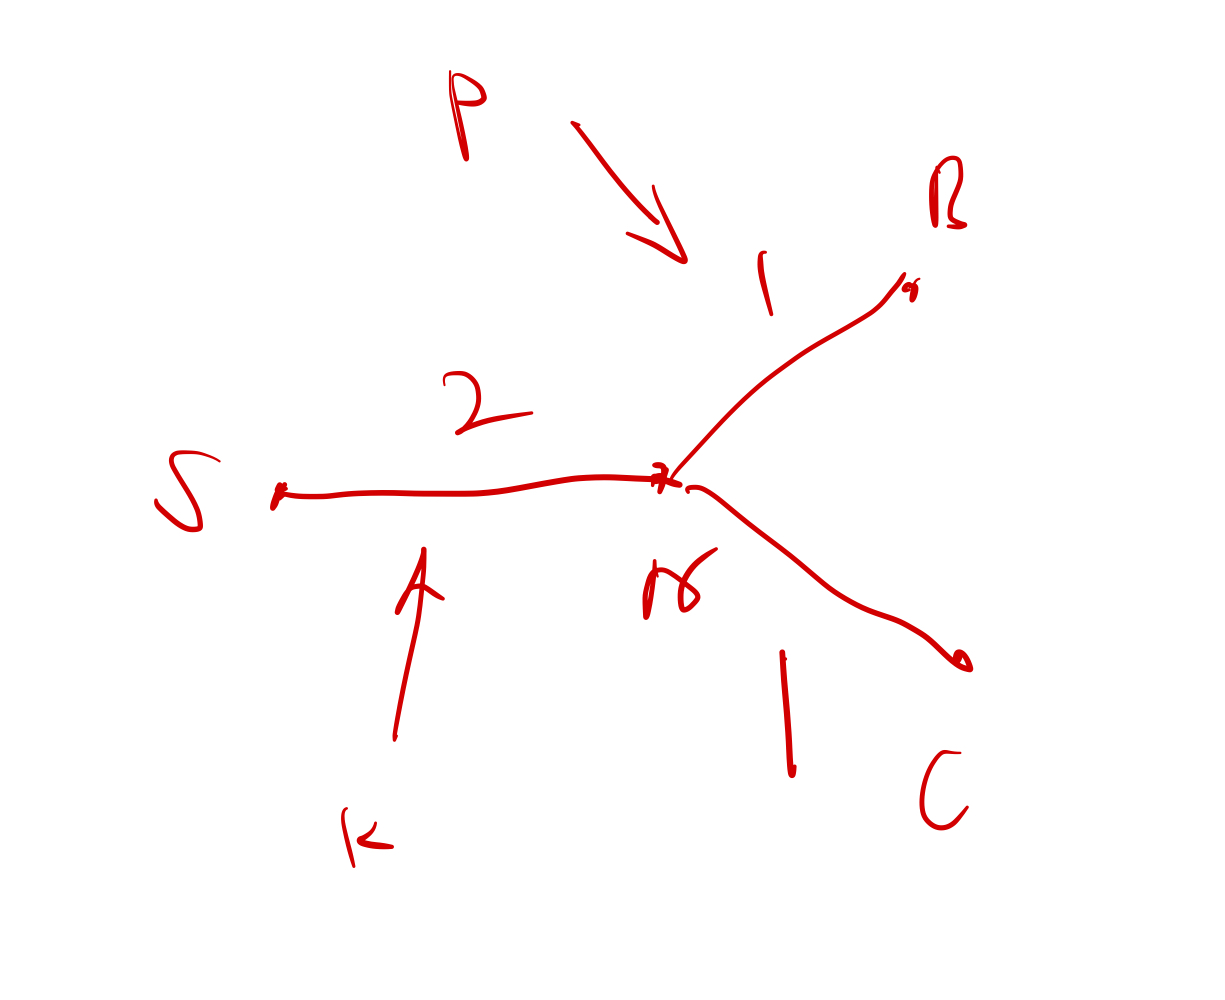
\includegraphics[width=0.4\textwidth]{p4.jpeg}
    \end{center} 

        \end{sol}
        \item Create a graph and give a Smallest Last Vertex Ordering where the terminal clique is not the largest clique in the graph. Give the smallest last vertex ordering and CIRCLE THE VERTEX YOU REMOVED FIRST IN THE ORDERING
        \begin{sol}
                \hspace*{\fill}
                \begin{center}
    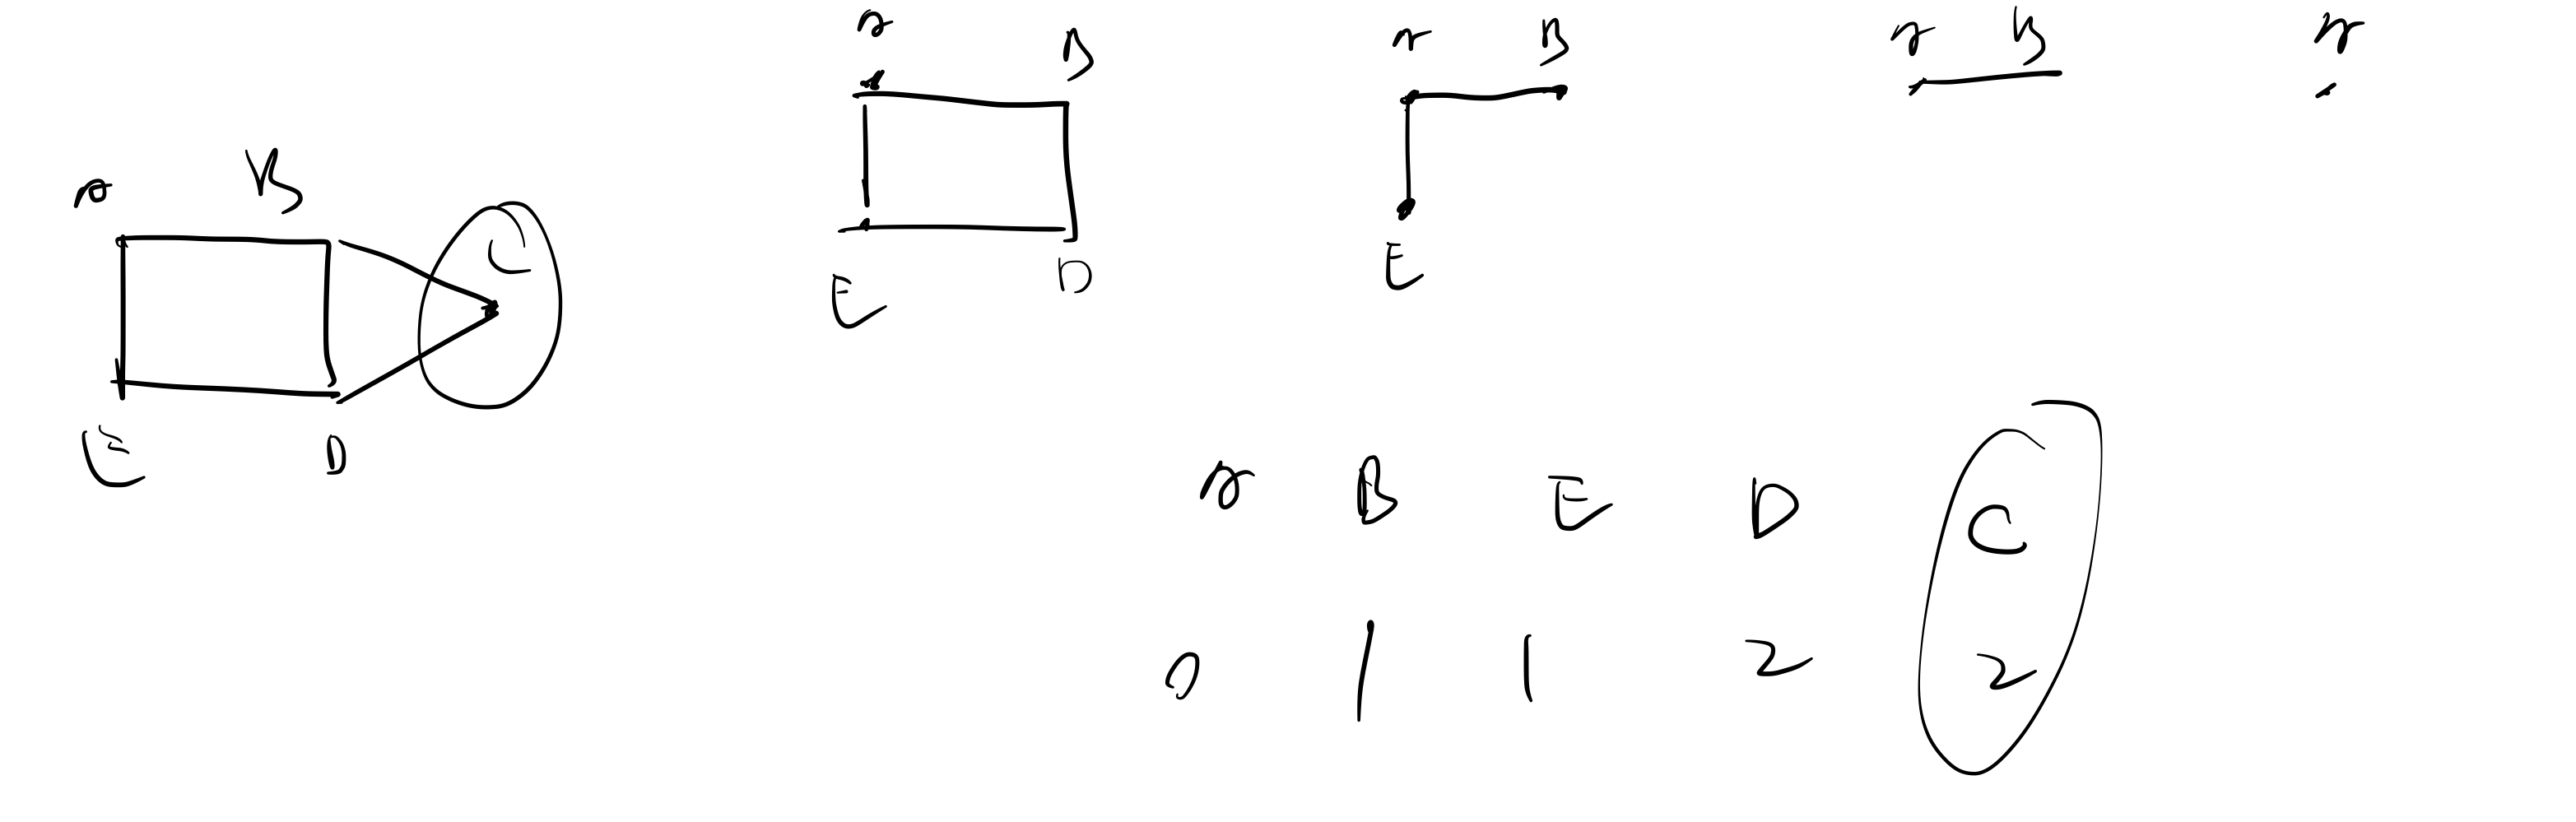
\includegraphics[width=0.6\textwidth]{p5.jpeg}
    \end{center} 
        \end{sol}
    \end{enumerate}

    \item \ [8 pts] Answer the following questions.:
    \begin{enumerate}
          \item A program requires 3s to brute force attack an encryption key of 128 bits. If
the running time is $\Theta(2^n)$ about how many years would it take to brute force attack an encryption key of 512 bits? (note there are about 32 million seconds in a year)
\begin{sol}
    \begin{align*}
        \frac{2^{512}}{2^{128}} \times 3 \times \frac{1}{32 \times 10^6} = 2 ^{379}\times 3 \times 10^{-6} \text{years}
    \end{align*}
\end{sol}
\item A program requires 3s to brute force attack an encryption key of 128 bits. If you have access to a quantum computer where the running time is $\Theta(n^2)$ about how many seconds would it take to brute force attack an encryption key of 512 bits?
\begin{sol}
    48s
\end{sol}

    \end{enumerate}


\item \ \textcolor{red}{[6 pts] Use the DGT algorithm discussed in class to determine how to represent the value 281.8 using the number system $\beta$=5, D = \{ -2, -1, 0, 1, 7 \}. Show your work. (Hint, 281.8 is 281 and 4/5 which can also be thought of as 282 and -1/5)}
\begin{sol}
    \begin{align*}
        0.\bar{1} = -1\times 5^{-1} = -\frac{1}{5}  \\
        -2 \bmod 5 = 3, -1 \bmod 5 = 4, 7 \bmod 5 = 2\\
    \end{align*}
    \begin{align*}
        & 282 \bmod 5 = 2 \rightarrow 7\\
        & 282 - 7 = 275 \\
        & 275 \div 5 = 55 \\
        & ----------------\\
        & 55 \bmod 5 = 0 \\
        & 55 - 0 = 55 \\
        & 55 \div 5 = 11 \\
        & ----------------\\
        & 11 \bmod 5 = 1 \\
        & 11 - 1 = 10\\
        & 10 \div 5 = 2\\
        & ----------------\\
        & 2 \bmod 5 = 2 \rightarrow 7 \\
        & 2 - 7 = -5\\
        & -5 \div 5 = -1\\
        & ---------------\\
        & -1 \bmod 5 = -1 \\
        & -1 - (-1) = 0\\
        \therefore \bar{1}7107.\bar{1}
    \end{align*}
\end{sol}

\item \ [6 pts] You have a tree with the following in-order and pre-order traversals. Draw the tree:
\begin{center}
IN ORDER: P M W S Z B A Q L R B T \\
PRE\_ORDER: P M L B S W Z Q A T R B
\end{center}
        \begin{sol}
        \hspace*{\fill}
                                    \begin{center}
    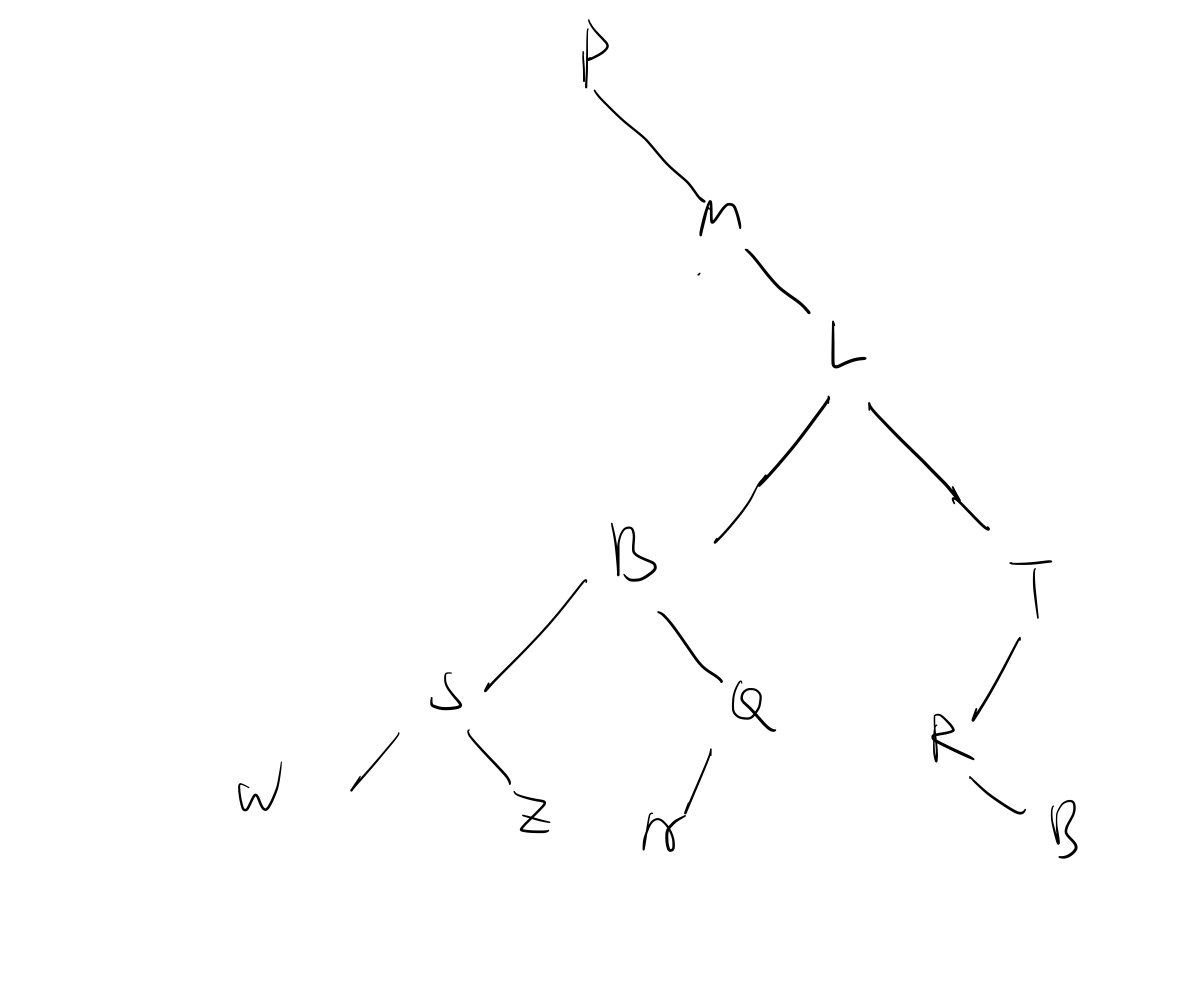
\includegraphics[width=0.6\textwidth]{p2.jpeg}
    \end{center} 
        \end{sol}


\item \ [8 pts] You have two strings, A and B.
\begin{itemize}
    \item String A has a length of 9.
    \item String B has a length of 7.
    \item String C has an unknown length.
    \item The Longest Common Subsequence between String A and C is 5.
\end{itemize}
\begin{enumerate}
    \item What is the minimum length of String C?
    \begin{sol}
        5
    \end{sol}
    \item What is the maximum length of String C?
    \begin{sol}
        infinitely
    \end{sol}
    \item What is the minimum length of the Levensthein Edit Distance of String A and String B
    \begin{sol}
        2
    \end{sol}
    \item What is the maximum length of the Levensthein Edit Distance of String A and String B?
    \begin{sol}
        9
    \end{sol}

\end{enumerate}


\item \ [8 pts] You are looking at a message and each symbol in a message that contains:
\begin{center}
    16 A's, 8 B's, 4 C's, 2 D's, 1 E's and 1 F's.
\end{center}

\begin{enumerate}
    \item How much entropy does each “B” have in the message?
    \begin{sol}
        2 bits
    \end{sol}
    \item How many bits of entropy are in the entire message?
    \begin{sol}
        62 bits
    \end{sol}
    \item Give a Huffman Coding of the symbols of the message?
            \begin{sol}
        \hspace*{\fill}
                                    \begin{center}
    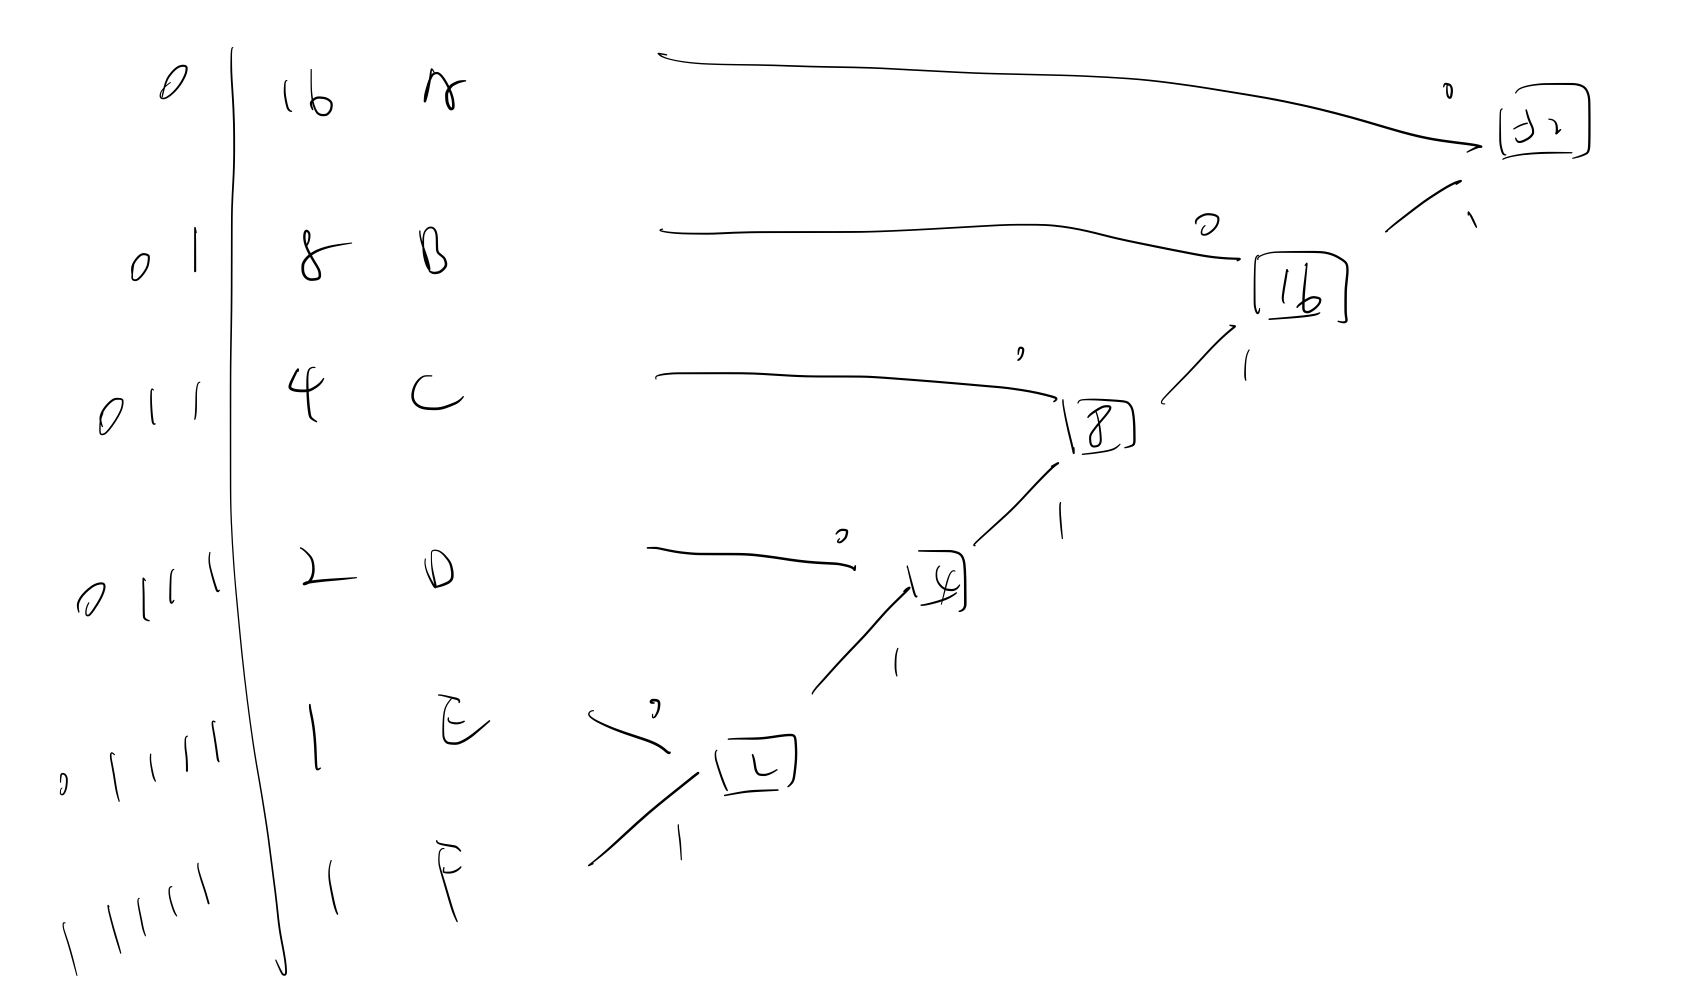
\includegraphics[width=0.8\textwidth]{p3.jpeg}
    \end{center} 
        \end{sol}
    \item How many bits are in the entire Huffman encoded message?
    \begin{sol}
        62 bits
    \end{sol}
\end{enumerate}

\end{enumerate}

\end{document}
